%%%%%%%%%%%%%%%%%%%%%%%%%%%%%%%%%%%%%%%%%%%%%%%%%%%%%%%%%%%%%%%%%%%%%%%%%%%%%%%%%%%%%%%%%%
% Based template: https://www.overleaf.com/latex/templates/uct-report-template/grctkzjtrqrm
%%%%%%%%%%%%%%%%%%%%%%%%%%%%%%%%%%%%%%%%%%%%%%%%%%%%%%%%%%%%%%%%%%%%%%%%%%%%%%%%%%%%%%%%%%
\documentclass[12pt]{article}
\usepackage[spanish]{babel}
\usepackage{natbib}
\usepackage{url}
\usepackage[utf8x]{inputenc}
\usepackage{amsmath}
\usepackage{graphicx}
\usepackage{float}
\usepackage{parskip}
\usepackage{fancyhdr}
\usepackage{vmargin}
\usepackage{listings}
\usepackage{xcolor}

\lstset{
  language=C,
  basicstyle=\ttfamily,
  backgroundcolor=\color{black!5},
  keywordstyle=\color{blue}\ttfamily,
  stringstyle=\color{red}\ttfamily,
  commentstyle=\color{green}\ttfamily,
  morecomment=[l][\color{magenta}]{\#}
}

\setmarginsrb{3 cm}{2.5 cm}{3 cm}{2.5 cm}{1 cm}{1.5 cm}{1 cm}{1.5 cm}

\title{DFPGA - ''Discrete FPGA''} % Title
\author{Aguilar Enriquez, Paul Sebastian \\ Cabrera Lopez, Oscar Emilio}  % Author
\date{\today} % Date

\makeatletter
\let\thetitle\@title
\let\theauthor\@author
\let\thedate\@date
\makeatother

\pagestyle{fancy}
\fancyhf{}
\rhead{\theauthor}
\lhead{\thetitle}
\cfoot{\thepage}

\begin{document}

%%%%%%%%%%%%%%%%%%%%%%%%%%%%%%%%%%%%%%%%%%%%%%%%%%%%%%%%%%%%%%%%%%%%%%%%%%%%%%%%%%%%%%%%%
\begin{titlepage}
    \centering
    
    \par
    \raisebox{-.5\height}{
\includegraphics[width=4cm]{escudo-unam.png}} % University Logo
    \hfill
    \raisebox{-.5\height}{
\includegraphics[width=4cm]{escudo-unam.png}} % Faculty Logo
    \par
    
    \hfill \break
    
    \textsc{\LARGE Universidad Nacional Autónoma de México}\\[2.0 cm]   % University Name
    \textsc{\Large Facultad de Ingeniería}\\[0.5 cm]                    % Course Code
    \textsc{\large Diseño de Sistemas Digitales}\\[0.5 cm]              % Course Name
    \rule{\linewidth}{0.2 mm} \\[0.4 cm]
    { \huge \bfseries \thetitle}\\
    \rule{\linewidth}{0.2 mm} \\[1.5 cm]
    
    \begin{minipage}{0.4\textwidth}
        \begin{flushleft} \large
            \emph{Integrantes:}\\
            \theauthor
        \end{flushleft}
    \end{minipage}~
    \begin{minipage}{0.4\textwidth}
        \begin{flushright} \large
            \emph{Codigo de Cuenta:} \\
            415028130\\312333261                                   % Your Student Number
        \end{flushright}
    \end{minipage}\\[2 cm]
    
    \begin{minipage}{0.4\textwidth}
        \begin{flushleft} \large
            \emph{Profesor:}\\
            M.I. Vicente Flores Olvera
        \end{flushleft}
    \end{minipage}~
    \begin{minipage}{0.4\textwidth}
        \begin{flushright} \large
            \emph{Fecha de entrega:}\\
            {\large \thedate}\\[2 cm]
        \end{flushright}
    \end{minipage}\\[2 cm]
    
    
    %{\large \thedate}\\[2 cm]
 
    \vfill
    
\end{titlepage}

%%%%%%%%%%%%%%%%%%%%%%%%%%%%%%%%%%%%%%%%%%%%%%%%%%%%%%%%%%%%%%%%%%%%%%%%%%%%%%%%%%%%%%%%%

\tableofcontents
\pagebreak

%%%%%%%%%%%%%%%%%%%%%%%%%%%%%%%%%%%%%%%%%%%%%%%%%%%%%%%%%%%%%%%%%%%%%%%%%%%%%%%%%%%%%%%%%

\section{Descripción del problema}

Implementar un FPGA con lógica  discreta utilizando completamente circuitos integrados de la familia 74XXX.

\section{Teoría}

\subsection{Definición de FPGA}
Los FPGA (Field Programmable Gate Arrays) son dispositivos prefabricados que pueden ser programados eléctricamente en al momento para convertirse en casi cualquier tipo de circuito o sistema digital. Para producciones de volumen bajo a medio, los FPGAs ofrecen soluciones más baratas y un tiempo de comercialización más rápido en comparación con los Circuitos Integrados de Aplicación Específica (ASIC), que normalmente requieren una gran cantidad de recursos en términos de tiempo y dinero para obtener el primer dispositivo. Los FPGAs por otro lado toman menos de un minuto para configurar y suelen tener un costo economico menor. También para diversos requisitos, una parte del FPGA se puede reconfigurar parcialmente mientras que el resto del FPGA sigue funcionando. Cualquier actualización futura en el producto final se puede actualizar fácilmente simplemente descargando un nuevo flujo de bits que representan la aplicación. La principal ventaja de los FPGAs es la flexibilidad.

La naturaleza flexible de los FPGAs los hace significativamente más grandes, más lentos y consumen más energía que sus equivalentes ASIC. Los FPGAs presentan una alternativa convincente para la implementación de sistemas digitales debido a su menor tiempo de comercialización y bajo costo de volumen.

Normalmente los FPGAs se comprenden de:
 \begin{itemize}
   \item Bloques lógicos programables que implementan funciones lógicas.
   \item Enrutamiento programable que conecta estas funciones lógicas.
   \item Bloques de E/S que están conectados a bloques lógicos a través de la interconexión de enrutamiento y que hacen conexiones tipo off-chip.
 \end{itemize}

Un ejemplo generalizado de un FPGA se muestra en la Fig. \ref{fig:1} donde los bloques lógicos configurables (CLBs) están dispuestos en una rejilla bidimensional y están interconectados por recursos de enrutamiento programables. Los bloques de E/S están dispuestos en la periferia de la rejilla y también están conectados a la interconexión de enrutamiento programable. El término ''programable/reconfigurable'' en FPGAs indica su capacidad para implementar una nueva función en el chip después de su fabricación. La reconfigurabilidad/programación de un FPGA se basa en una tecnología de programación subyacente, que puede causar un cambio en el comportamiento de un chip pre-fabricado después de su fabricación.


\begin{figure}[H]
  \centering
  %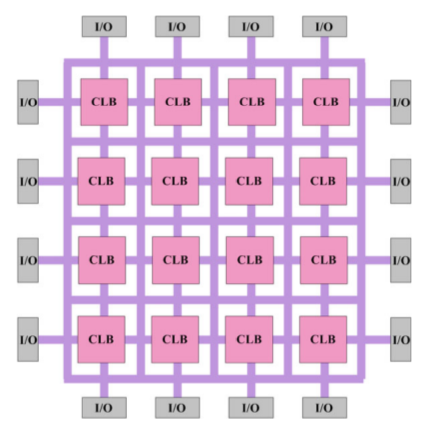
\includegraphics[height=5.5cm]{1-Overview-of-FPGA-architecture.png}
  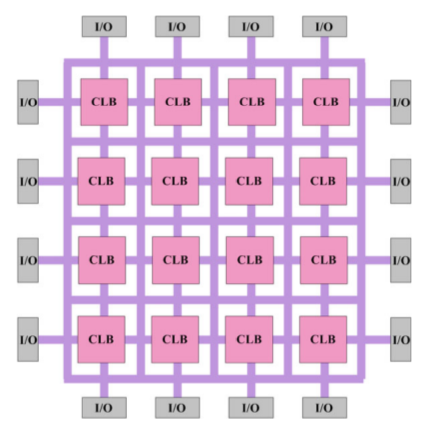
\includegraphics[]{1-Overview-of-FPGA-architecture.png}
  \caption{Vista de la arquitectura básica de un FPGA.}
  \label{fig:1}
\end{figure}

\subsection{Bloque lógico configurable}

Un bloque lógico configurable (CLB) es un componente básico de un FPGA que proporciona la lógica básica y la funcionalidad de almacenamiento para el diseño de la aplicación objetivo. Con el fin de proporcionar la lógica básica y la capacidad de almacenamiento, el componente básico puede ser un transistor o un procesador entero. Sin embargo, estos son los dos extremos donde en un extremo el componente básico es de grano fino (en el caso de transistores) y requiere una gran cantidad de interconexión programable que finalmente resulta en un FPGA que sufre ineficiencia de área, bajo rendimiento y alta potencia consumo. En el otro extremo (en el caso del procesador), el bloque lógico básico es muy grueso y no se puede usar para implementar pequeñas funciones ya que conducirá a desperdicio de recursos.

Entre estos dos extremos, existe un espectro de bloques lógicos básicos. Algunos de ellos incluyen bloques lógicos que están hechos de puertas NAND, una interconexión de multiplexores, tabla de consulta (Lookup Table - LUT) y puertas de entrada ancha de estilo PAL. Los vendedores comerciales como Xilinx y Altera utilizan CLBs basados ​​en LUT para proporcionar lógica básica y funcionalidad de almacenamiento. Los CLBs basados ​​en LUT proporcionan un buen equilibrio entre los bloques lógicos de grano demasiado fino y demasiado grueso. Un CLB puede comprender un único elemento lógico básico (Basic Logic Element - BLE), o un grupo de BLEs interconectadas localmente (como se muestra en la figura \ref{fig:2}). Un BLE simple consiste en un LUT, y un flip-flop. Un LUT con \textit{k} entradas (LUT-k) contiene $2^{k}$ bits de configuración y puede implementar cualquier función booleana de k-entradas. La Figura \ref{fig:3} muestra un BLE simple que comprende un LUT de 4 entradas (LUT-4) y un Flip-Flop de tipo D. El LUT-4 utiliza 16 bits SRAM para implementar cualquier función booleana de 4 entradas. La salida de LUT-4 está conectada a un Flip-Flop opcional. Un multiplexor selecciona la salida BLE para ser la salida de un flip-flop o el LUT-4.

\begin{figure}[H]
  \centering
  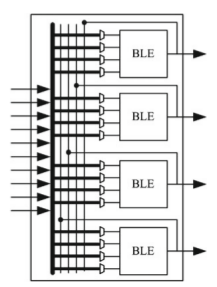
\includegraphics[]{2-CLB-having-four.png}
  \caption{Bloque lógico configurable (CLB) con cuatro BLEs}
  \label{fig:2}
\end{figure}

\begin{figure}[H]
  \centering
  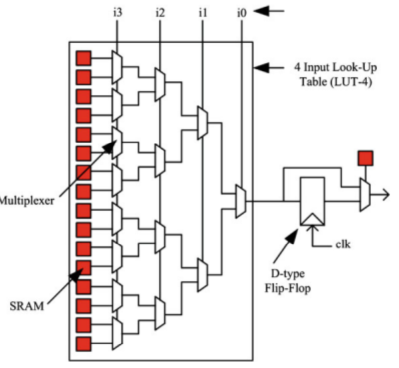
\includegraphics[height=8cm]{3-Basic-logic-element.png}
  \caption{Bloque lógico configurable (CLB) básico}
  \label{fig:3}
\end{figure}

\subsection{Arquitecturas de enrutamiento FPGA}

En un FPGA, la funcionalidad de cálculo es proporcionada por sus bloques lógicos programables y estos bloques se conectan entre sí a través de la red de enrutamiento programable. Esta red de encaminamiento programable proporciona conexiones de enrutamiento entre bloques lógicos y bloques de E/S para implementar cualquier circuito definido por el usuario.

La interconexión de enrutamiento de un FPGA consiste en cables y interruptores programables que forman la conexión requerida. Estos interruptores programables se configuran utilizando la tecnología programable.


Dado que las arquitecturas FPGA afirman ser un candidato potencial para la implementación de cualquier circuito digital, su interconexión de enrutamiento debe ser muy flexible para que puedan acomodar una amplia variedad de circuitos con demandas de enrutamiento muy variadas. Aunque los requerimientos de enrutamiento varían de circuito a circuito, ciertas características comunes de estos circuitos pueden usarse para diseñar óptimamente la interconexión de enrutamiento de la arquitectura FPGA.

Por ejemplo, la mayoría de los diseños muestran localidad, por lo que requieren abundantes cables cortos. Pero al mismo tiempo hay algunas conexiones distantes, lo que lleva a la necesidad de cables largos y escasos. Por lo tanto, el cuidado debe tenerse en cuenta al diseñar la interconexión de enrutamiento para las arquitecturas FPGA donde tenemos que abordar la flexibilidad y la eficiencia. La disposición de recursos de encaminamiento, relativa a la disposición de bloques lógicos de la arquitectura, juega un papel muy importante en la eficiencia global de la arquitectura. Esta disposición se denomina aquí como arquitectura de enrutamiento global, mientras que los detalles microscópicos relativos a la topología de conmutación de diferentes bloques de conmutación se denominan arquitectura de enrutamiento detallada. Sobre la base de la disposición global de los recursos de enrutamiento de la arquitectura, las arquitecturas FPGA pueden clasificarse como de tipo jerárquico o de isla, no se abundara en los calsificaciones.

\begin{figure}[H]
  \centering
  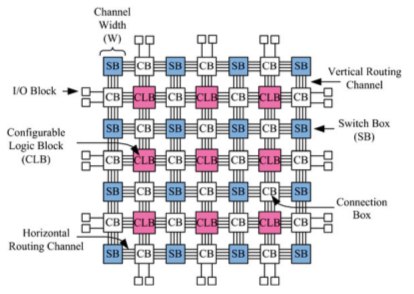
\includegraphics[]{4-Overview-of-mesh-based-FPGA-architecture.png}
  \caption{Vista de la arquitectura de un FPGA basado en malla.}
  \label{fig:4}
\end{figure}

\subsection{Arquitectura Asíncrona FPGA}

Otro enfoque alternativo que se ha propuesto para mejorar el rendimiento general de la arquitectura FPGA es el uso de elementos de diseño asíncrono.

Convencionalmente, los circuitos digitales están diseñados para la operación síncrona ya su vez las arquitecturas FPGA se han centrado principalmente en la implementación de circuitos síncronos. Se proponen diseños asíncronos para mejorar la eficiencia energética de los FPGA asincrónicos, ya que los diseños asíncronos ofrecen energía potencialmente menor, ya que la energía se consume sólo cuando sea necesario. También las arquitecturas asíncronas pueden simplificar el proceso de diseño ya que las complejas redes de distribución de reloj se vuelven innecesarias.

\subsection{Programación}

En el FPGA no se realiza programación tal cual como se realiza en otros dispositivos como DSP, CPLD o microcontroladores. El FPGA tiene celdas que se configuran con una función específica ya sea como memoria (FLIP-FLOP tipo D), como multiplexor o con una función lógica tipo AND, OR, XOR. La labor del ''programador'' es describir el hardware que tendrá la FPGA. 

El diseñador cuenta con la ayuda de entornos de desarrollo especializados en el diseño de sistemas a implementarse en un FPGA. Un diseño puede ser capturado ya sea como esquemático, o haciendo uso de un lenguaje de programación especial. Estos lenguajes de programación especiales son conocidos como HDL o Hardware Description Language (lenguajes de descripción de hardware). Los HDLs más utilizados son:

\begin{itemize}
  \item VHDL
  \item Verilog
  \item ABEL
\end{itemize}

En un intento de reducir la complejidad y el tiempo de desarrollo en fases de prototipaje rápido, y para validar un diseño en HDL, existen varias propuestas y niveles de abstracción del diseño. Los niveles de abstracción superior son los funcionales y los niveles de abstracción inferior son los de diseño al nivel de componentes hardware básicos.

\section{Método de solución}

\subsection{Introducción}

Durante la investigación de la arquitectura de un FPGA nos dimos cuenta que su implementación es relativamente sencilla dado que su diseño puede implementarse de manera modular, sin embargo el lograr un diseño adecuado es un reto que implica una variedad de consideraciones.  

Dentro de las consideraciones necesarias esta el diseño de cada elemento como los son los bloques lógicos programables, el sistema de enrutamiento, los segmentos de E/S. A su vez es necesario considerar el tipo de elemento que se usara como memoria para almacenar el programa que el FPGA ejecutara, esto a la vez implica que para la creación del programa se requiere a su vez el diseño e implementación de un lenguaje de programación tipo HDL y todo lo que esto implica (un compilador o interprete, reglas de sintaxis, semántica, que el lenguaje se adapte a la arquitectura del FGPA, etc.). 
 
Dadas todas las consideraciones anteriores, el diseño de un FPGA y todo su entorno se vuelve una tarea extensa que puede sobrepasar el alcance de la materia para la cual se piensa realizar este proyecto, por lo que hemos decidido (y con aprobación del profesor correspondiente) apoyarnos en un diseño encontrado previamente, el cual implementa en su totalidad elementos vistos en clase, los cuales permiten que el diseño sea apropiado para la materia.  

De forma concluyente, este proyecto se considera como una extensión a modo de análisis de estudio del sobre el proyecto en el cual se basa, dado que el proyecto original es una buena implementación de un FPGA pero que desafortunadamente no se encuentra lo suficientemente documentado y explicado, este documento trata de abordar de la mejor manera posible el diseño e implementación original, así como la integración de elementos faltantes en las fuentes compartidas por el autor.

\subsection{Planteamiento de diseño}

\subsubsection{CLB y LUT}

El bloque de construcción más básico de un FPGA es la celda o ''slice'', a la cual en la teoría hemos referido como CLB. Normalmente, un CLB tiene algunas entradas, una tabla de búsqueda (LUT) que se puede programar para evaluar cualquier función booleana sobre esas entradas y una o más salidas, cada una de las cuales se puede configurar para actualizar inmediatamente cuando la entrada se actualiza (Asíncrono) o actualizar sólo en la siguiente marca de reloj, utilizando un flip-flop integrado en el segmento (Síncrono). 
 
El núcleo de un CLB, la tabla de búsqueda, se puede programar para evaluar cualquier función booleana en ella y la salida del resultado. Su implementación es muy simple, y es una técnica también utilizada para implementar micro código y otra lógica de encolado configurable. En principio, lo que haces es esto: tomar un IC de memoria como un SRAM o una EEPROM y conectar las líneas de dirección a sus entradas, y las líneas de datos a su salida. Ahora, cualquier combinación de estados de entrada se interpretará como una dirección, que la memoria buscará y proporcionará en las salidas de datos. Mediante la programación de la memoria con las tablas de estado para las funciones que desea calcular, puede configurarlo para evaluar lo que quiera. 
 
Desafortunadamente, ninguna de las memorias de la serie 74XXX se fabricada actualmente, y aunque hay un montón de SRAMs y EEPROMs disponibles, los tamaños más pequeños disponibles son significativamente más grandes de lo que queremos para un simple FPGA discreto. Además, para poder programar y leer la memoria, necesitaríamos mucha lógica para cambiar entre escribir en la memoria y leer de ella (en una memoria de ''puerto único'', éstos usan los mismos pines). 
 
Sin embargo, una solución simple se presenta: registros de desplazamiento. Un registro de desplazamiento es efectivamente una memoria de 8 bits, con entradas en serie y cada bit expuesto en su propio pin. Combinando esto con un multiplexor de 8 vías, tenemos una LUT básica de 3 entradas de 1 salida. Nuestro LUT se puede reprogramar utilizando los datos, el reloj y las líneas de cierre, y muchos de ellos pueden encadenarse y programarse en serie. Las 3 entradas de selección en el mux de 8 vías forman las entradas al LUT, y el bit de salida del mux es la salida. Por lo tanto, en dos CI de la serie 74XXX disponibles, tenemos una tabla de búsqueda completa.  
 
Para nuestro CLB de FPGA, utilizaremos dos de estos LUTs discretos, con sus entradas unidas entre sí. ¿Por qué dos? Porque una capacidad combinada de 3 entradas y 2 salidas sobre el más pequeño puede implementar cosas interesantes con 3 entradas y 2 salidas se permite construir un sumador completo en una sola celda. Cualquier cantidad menor de entradas o salidas limita severamente nuestras capacidades.

\subsubsection{Arquitectura Sincrona/Asíncrona}

El siguiente componente son los flipflops y la lógica para seleccionar el modo asíncrono o síncrono. Hay una gran variedad de flipflops y registros disponibles, de 2 a 8 en un único IC, y con varios métodos de control, por lo que no hay problema. Elegir entre síncrono y asincrónico es un poco más difícil. La elección natural aquí es un multiplexor de 2 vías, pero mientras existen chips con múltiples multiplexores de 2 vías, todas juntan las líneas de selección, lo que significa que debe elegir la misma entrada para todos los multiplexores en un chip. Obviamente, esto no es realmente adecuado para nuestra aplicación.

Afortunadamente, un multiplexor de 2 vías no es difícil de construir. Hay varias opciones, pero la más eficiente es usar bufferes de tres estados. Hay un par en la gama 7400 - el 74**125 y el 74**126 que resuelven nuestros requisitos. Cada uno contiene cuatro búferes de tres estados, la única diferencia entre los dos chips es que uno habilita su salida cuando la línea de habilitación es alta, mientras que el otro permite su salida cuando es baja. Al unir estos juntos en pares, podemos crear multiplexores, cada IC nos brinda cuatro multiplexores independientes. Dos multiplexores más un registro nos consigue nuestra lógica de selección de sincrona/asíncrona. Necesitamos una forma de controlar los multiplexores, por lo que una poner en cadena en otro registro de desplazamiento nos permite programarlos. 

\subsubsection{Enrutamiento}

El enrutamiento flexible es un atributo clave de cualquier FPGA útil, sin un buen enrutamiento, no se pueden obtener señales donde tienen que ir y perder recursos preciosos, por lo que el FPGA mucho menos útil. El enrutamiento, sin embargo, utiliza una gran cantidad de recursos para implementar correctamente. 
 
Típicamente, los FPGAs colocan las CLBs individuales en una rejilla rectangular. Los buses funcionan entre los CLBs en forma de rejilla horizontalmente y verticalmente. Una CLB es capaz de aprovechar algún subconjunto de las líneas en su intersección. Típicamente, el bus puede continuar a través de una CLB ininterrumpidamente, o el bus se puede romper, creando buses separados a cada lado de la CLB. En algunos casos, los buses también pueden conectarse entre sí de otras maneras, encaminándose entre líneas de bus diferentes o entre buses horizontales y verticales sin partir directamente la CLB. 
 
Los buses de un bit son un poco estrechos, incluso para nuestro propósito, aplicaciones interesantes van a requerir más que eso, así que se proponen buses de 2 bits, tanto vertical como horizontal. Muchos FPGAs incluyen buses en una dirección u otra, esto ahorra recursos de enrutamiento, favoreciendo usos más comunes a expensas de hacer configuraciones menos comunes más caras. En nuestro caso, facilitaremos la lectura de los buses ''izquierdo'' y ''superior'' y la escritura en los buses ''derecho'' e ''inferior''. Podemos hacer esto teniendo multiplexores de 2 entradas en cada uno de los buses izquierdo, superior y derecho, estos multiplexores se alimentan en las 3 entradas de nuestra LUT. Para la salida, podemos usar más buffers de tres estados para permitir que una LUT emita en una o ambas líneas del bus derecho, mientras que la otra sale a una o a ambas líneas de bus inferior. Para leer desde la parte inferior, o para conducir las líneas izquierda o superior, simplemente hay que conducir al lado opuesto, y cerrar el interruptor de bus apropiado. 
 
Para los interruptores de bus, se usara la configuración más simple: un interruptor que conecta cada una de las líneas superior e inferior, y un interruptor que conecta cada una de las líneas izquierda y derecha, que se puede abrir o cerrar individualmente. El CI 74**4066 es un ''conmutador bilateral cuádruple'' que proporciona una manera conveniente de hacer esto en un solo CI. Todo el enrutamiento implica 3 bits para los multiplexores de entrada, 4 bits para la salida habilitada, y 4 bits más para los interruptores de bus, por lo que vamos a utilizar otro registro de desplazamiento y algunos de los bits sobrantes de otro registro que hemos añadido para la selección síncrona/asíncrona.

\subsubsection{Componentes a utilizar}

Con el diseño anterior, se llega a que se necesitan los siguientes componentes. 
 
\begin{itemize} 
  \item 4 x 74HC595 Registros de desplazamiento, para LUTs y estado de enrutamiento/multiplexor. 
  \item 2 x 74HC251 multiplexor de 8 líneas, para LUTs. 
  \item 2 x 74HC125 y 2 x 74HC126 búferes de tres estados, para multiplexores y salida habilitada. 
  \item 1 x 74HC173 Registro de 4 bits, para funcionamiento síncrono. 
  \item 1 x 74HC4066 Interruptor Cuádruple Bilateral, para interruptores de buses. 
\end{itemize} 
  
Se trata de un total de 12 CIs de lógica discreta para implementar una celda moderadamente. Se usara unos cuantos LEDs para dar un indicador visual del estado de las líneas de bus.

\section{Construcción Virtual}

\begin{figure}[H]
  \centering
  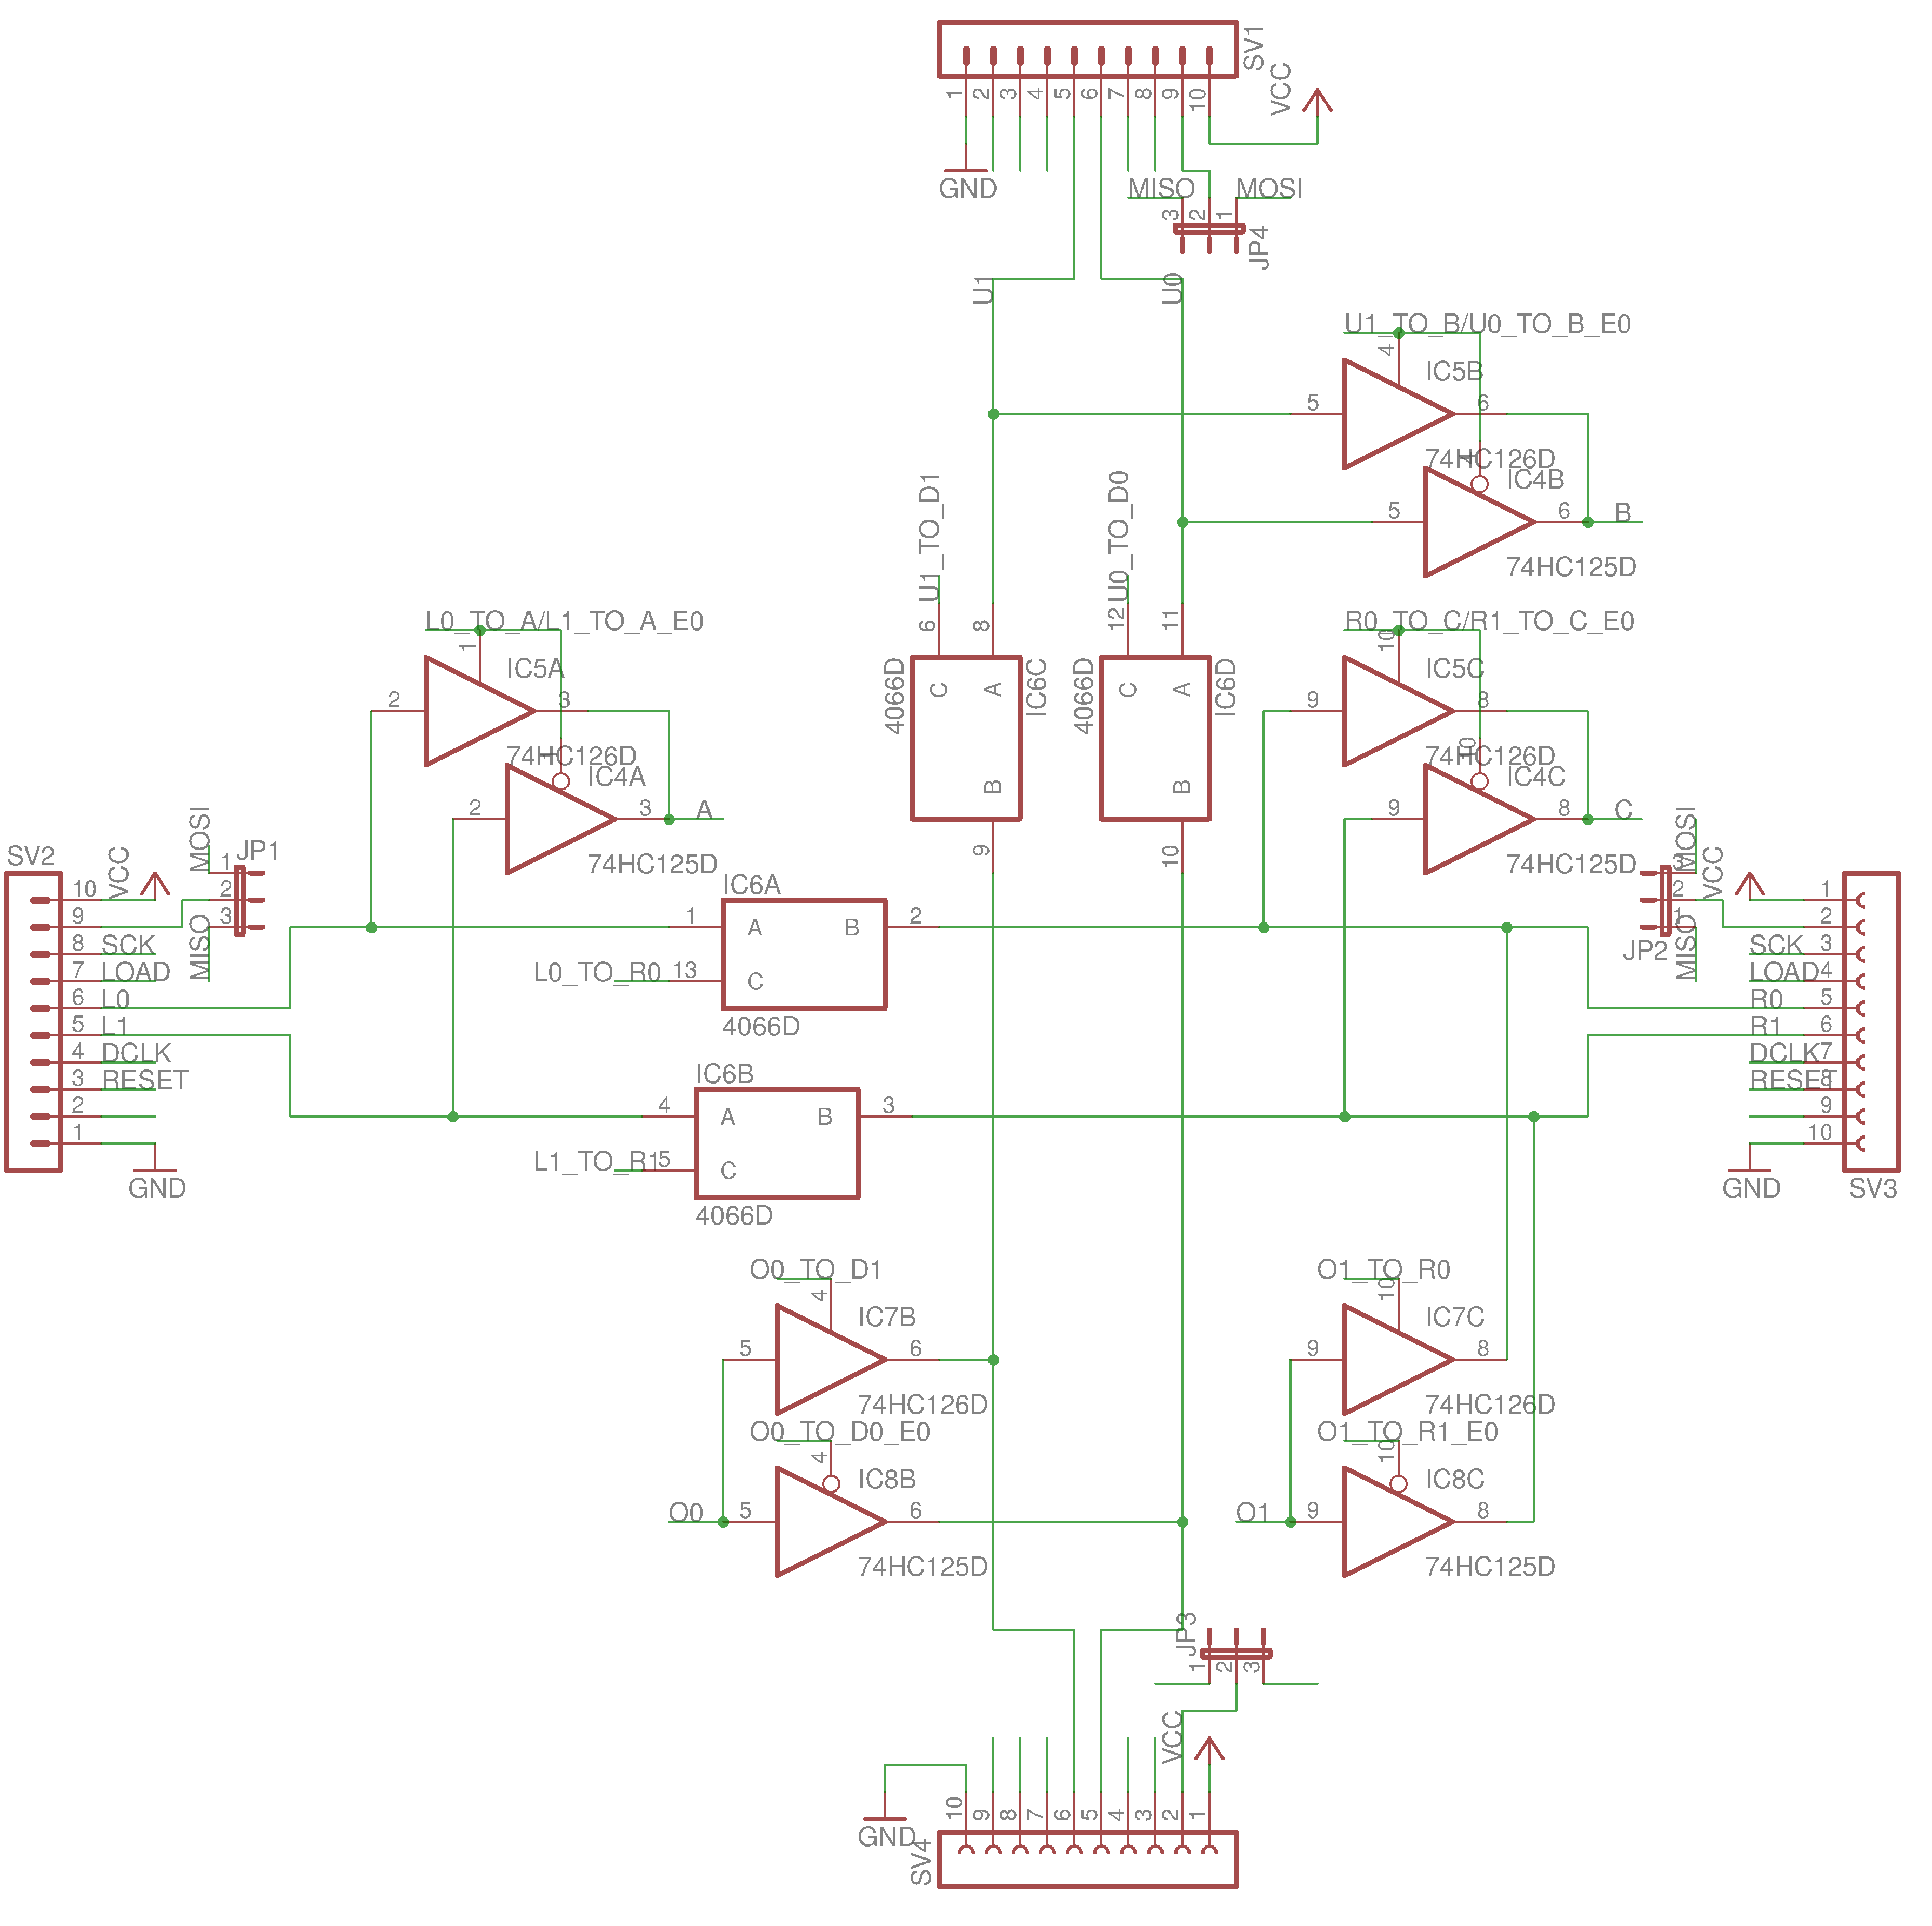
\includegraphics[width=\textwidth]{5-input-output-routing.png}
  \caption{Vista de la arquitectura de enrutamiento y E/S la celda del FPGA.}
  \label{fig:5}
\end{figure}

\begin{figure}[H]
  \centering
  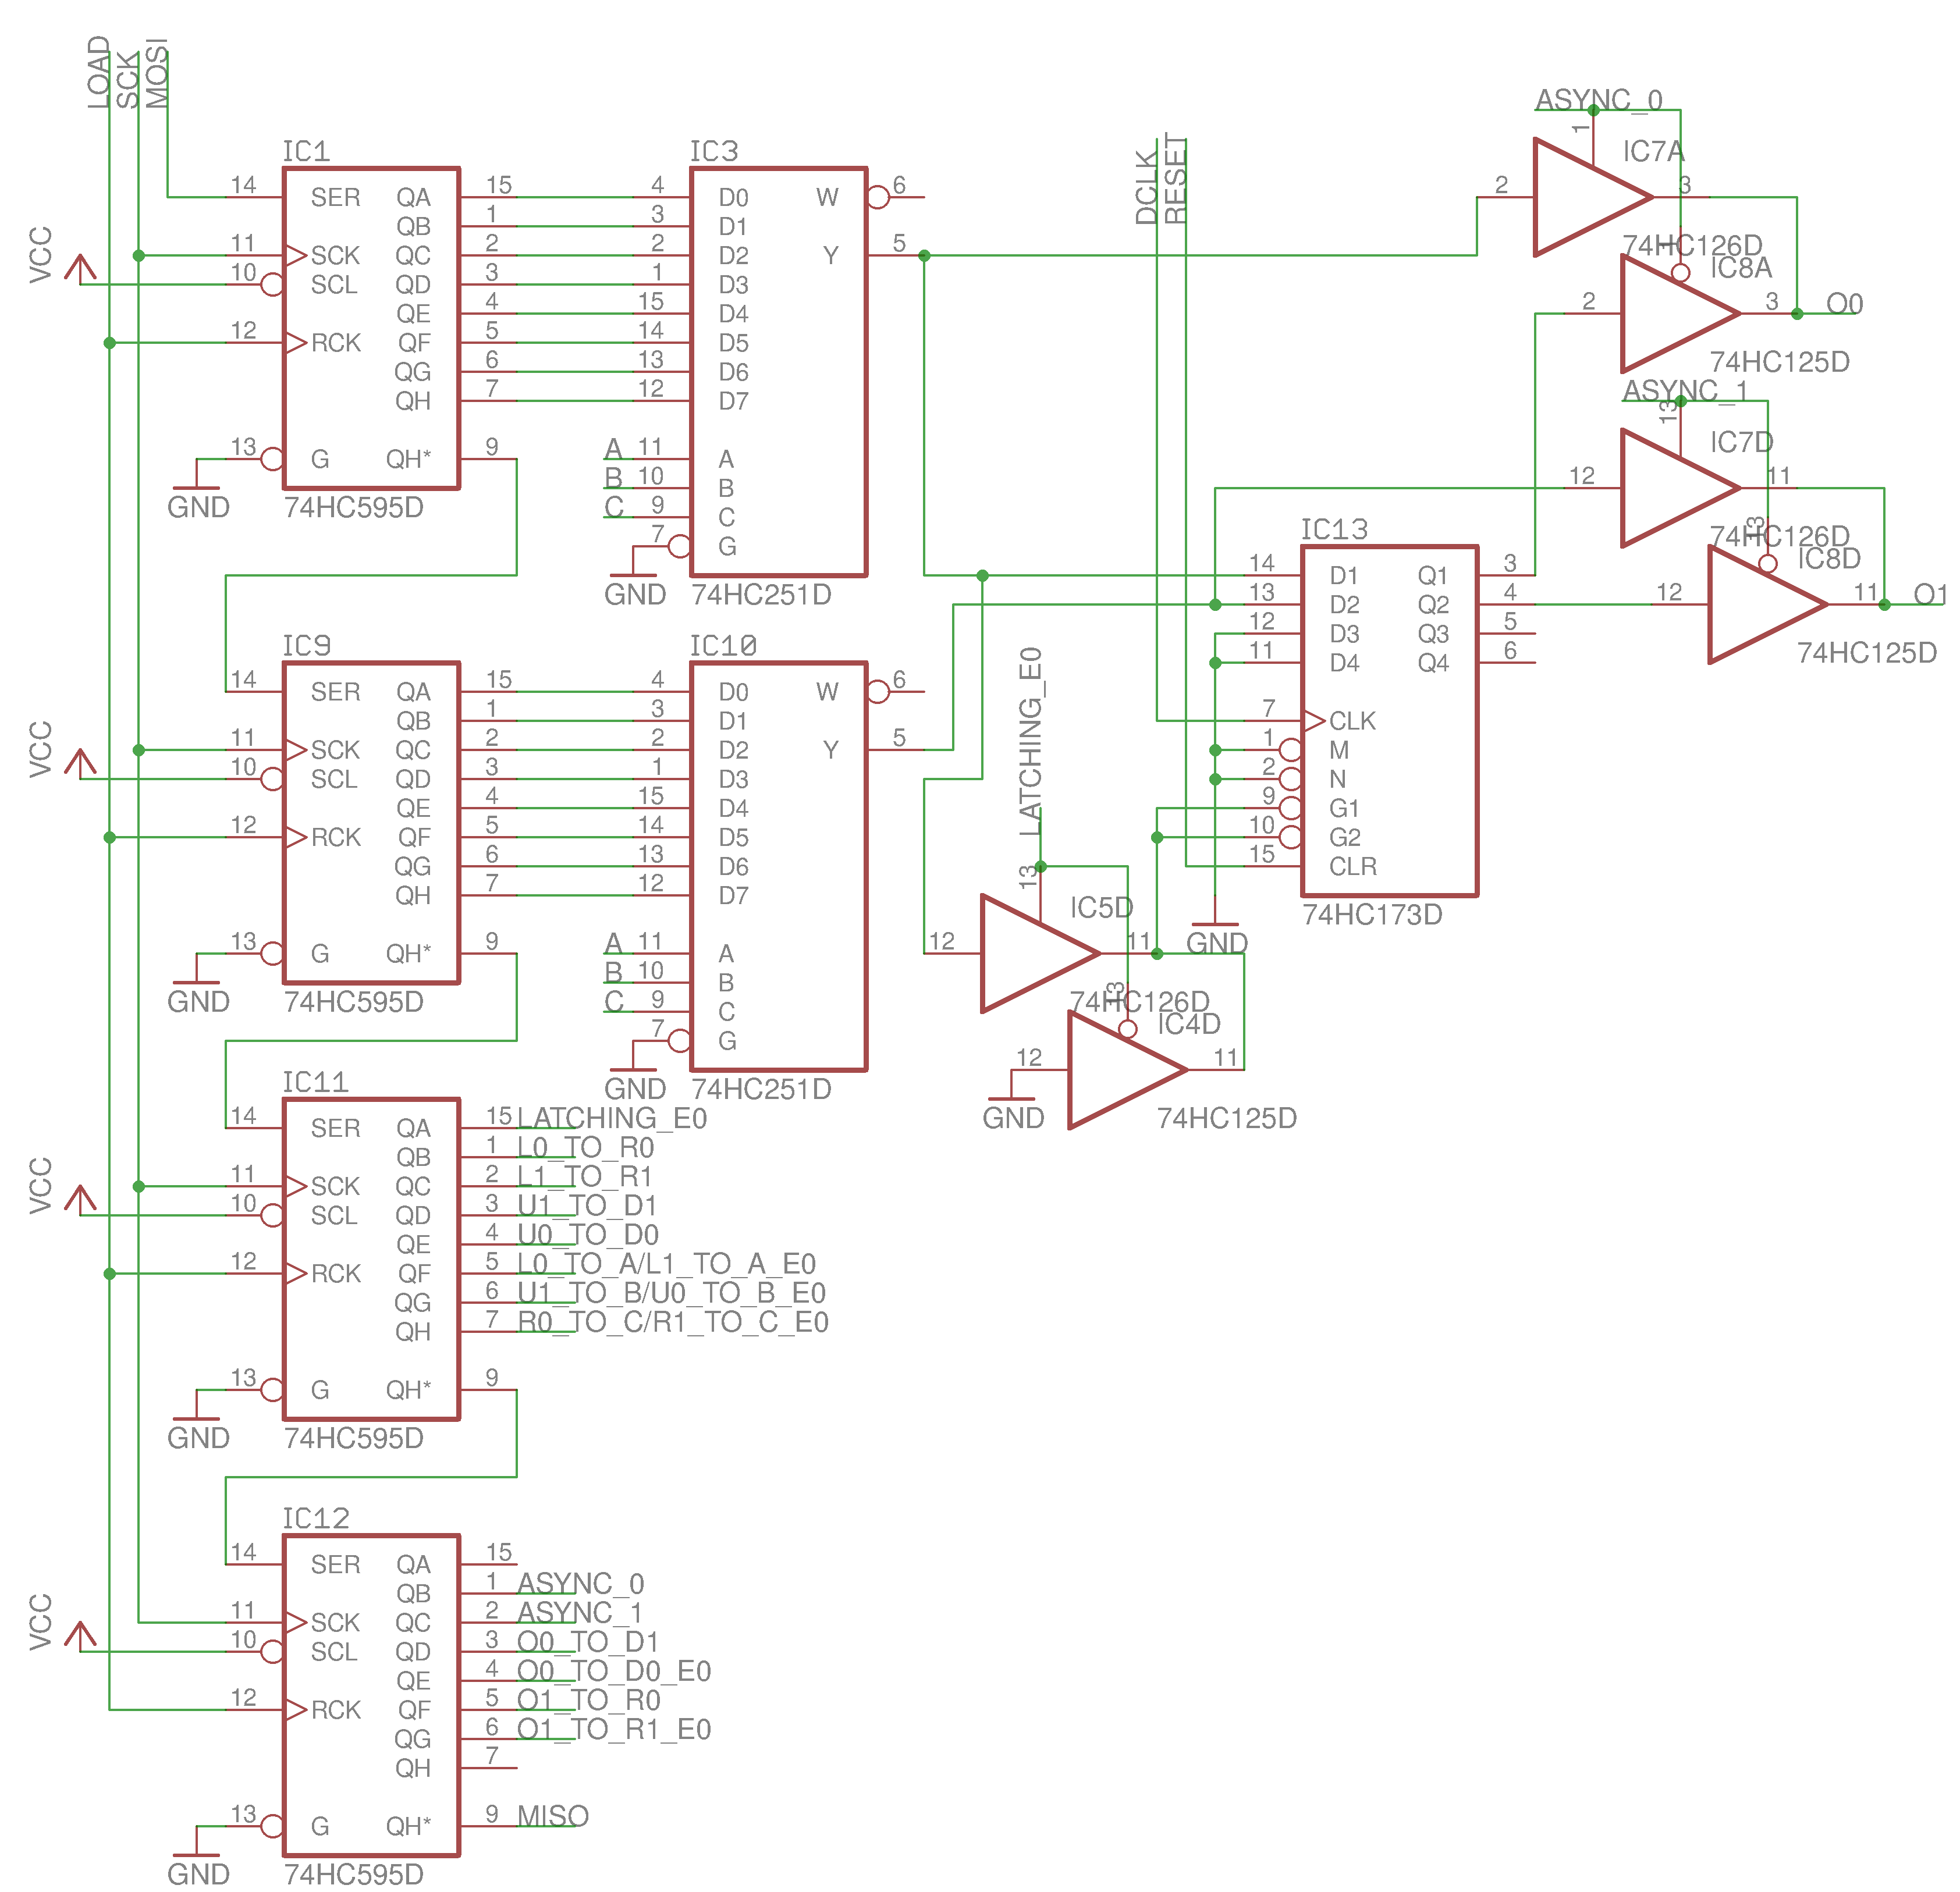
\includegraphics[width=\textwidth]{6-clb-lut.png}
  \caption{Vista de la arquitectura de la CLE, LUTs y método de sincronización.}
  \label{fig:5}
\end{figure}

\section{Código}

El autor del proyecto en los recursos y fuentes que libero no incluyo el código del programa para cargar la información en la celda diseñada, por lo que se implemento un programa en Arduino que permite el envió del programa en forma serial. 
 
Al utilizarse cuatro registros de corrimiento de 8 bits, el programa que se debe enviar a memoria es de 4 bytes. De los cuales 2 bytes son de control y los 2 restantes son para las LUTs. 
 
El código en Arduino es sencillo, envía de forma serial los datos, implementando un ciclo de reloj para enviar cada bit, esto se hace respetando las conexiones de los registros de corrimiento que están conectados a modo de expansión en serie.

\begin{lstlisting}
#include <Arduino.h>

/* 
 *  Basado en el codigo "shiftOutCode, Hello World" de Carlyn Maw y 
 *  Tom Igoe como ejemplo en el sitio oficial de Arduino.
*/

int dataPin = 9;    // Serial Data,  MOSI
int clockPin = 10;  // Clock para el serial,  SCK[1]
int dCLK = 11;      //  Clock general,  DCLK[2]
int latchPin = 12;  // Clock para los FF,   LOAD[3]
int clrFF = 13;     // Limpia los FF,  RESET[4]
byte dataArray[4];  // Data Array
byte data;          // Byte holder

void setup() {
    // Indicamos los pines como salida
    pinMode(latchPin, OUTPUT);
    pinMode(clockPin, OUTPUT);
    pinMode(dataPin, OUTPUT);
    pinMode(clrFF, OUTPUT);
    pinMode(dCLK, OUTPUT);

    // Programa que se enviara al FPGA
    dataArray[0] = 0x00;
    dataArray[1] = 0xff;
    dataArray[2] = 0x1c;
    dataArray[3] = 0x76;

     // Limpiamos los FF (clear)
    digitalWrite(clrFF, HIGH);
    // Enviaremos cuatro bytes
    for (int j = 0; j < 4; j++) {
        // Recuperamos el byte a enviar
        data = dataArray[j];
        // Ponemos en bajo el latch del registro para que no elimine 
        // los datos que apenas esta cargando
        digitalWrite(latchPin, LOW);
        // Enviamos el datos de forma serial comenzando por el bit 
        // mas significativo
        shiftOut(dataPin, clockPin, MSBFIRST, j);
        // Regresamos a alto el latch del registro dado que ya no esta 
        // escuchando
        digitalWrite(latchPin, HIGH);
        // Delay para dar tiempo de respuesta al circuito
        delay(10);
    }
    // Desactivamos la limpieza de los FF
    digitalWrite(clrFF, LOW);
    // Ponemos el reloj en cero
    digitalWrite(dCLK, LOW);
}

void loop() {
    // Switcheamos el bit del reloj cada segundo
    digitalWrite(dCLK, HIGH);
    delay(1000);
    digitalWrite(dCLK, LOW);
    delay(1000);
}
\end{lstlisting}

\bibliographystyle{plain}
\bibliography{biblist}

\end{document}
